\title{LearnReact:\\ An Interactive Tutorial}
\author{
        Barry Yang \\
        CS 191
}
\date{\today}

\documentclass[11pt]{article}
\usepackage{graphicx}
\usepackage[font=small,labelfont=bf]{caption}
\usepackage{times}
\usepackage{url}
\setlength{\oddsidemargin}{0in}
\setlength{\evensidemargin}{0in}
\setlength{\textwidth}{6.5in}
\setlength{\topmargin}{0in}
\setlength{\textheight}{8.5in}
\setlength{\headheight}{0pt}
\setlength{\headsep}{0pt}

\setcounter{topnumber}{3}%
\def\topfraction{.7}% 
\setcounter{bottomnumber}{1}
\def\bottomfraction{.3}
\setcounter{totalnumber}{5}%
\def\textfraction{.1}% was .2
\def\floatpagefraction{.7}% was .7
\setcounter{dbltopnumber}{2}
\def\dbltopfraction{.7}
\def\dblfloatpagefraction{.5}

\newcommand{\figcaption}[1]{\caption[]{#1}}
\newcommand{\figpart}[1]{\textbf{(#1)}\nolinebreak[4]\relax}
\newcommand{\figparts}[2]{\mbox{\textbf{(#1)--(#2)}}\nolinebreak[4]\relax}

\begin{document}
\maketitle

%\begin{abstract}
%This is the paper's abstract \ldots
%\end{abstract}

\section{Introduction}

Since being introduced in 2012, the React framework has made a big impact in the web development space. According to NPM Trends, React is the most popular frontend web development framework with 125 million downloads, ahead of the Angular framework with about 60 million downloads and the VueJS framework with about 20 million downloads \cite{popularity}.

Despite the framework's popularity, React has a steep learning curve. According to a survey sent out to Dartmouth's CS 52 web development class, fourteen out of twenty-two respondents indicated that they found learning React the hardest part of the course, despite an abundance of class support and online tutorials. After examining current online tutorials and interviewing students learning React, we noticed that many students did not understand basic concepts even after reading course materials or tutorials found online. Thus, we created \textit{LearnReact}, a tutorial that allowed students to learn React interactively, via modules that focus on specific concepts at a time. Another motivation for the application would be to create an application robust enough to be used in CS 52.

The interactive format of the tutorial, as well as motivation for the project, is inspired by Dartmouth College's \textit{Project Python} project \cite{pp}, which teaches basic computer science principles in an interactive way. The format of the app, which includes a table of contents that link to modules featuring a core concept, was directly inspired by the \textit{Project Python} project.

This paper will be organized as follows. Section 2 provides an overview of the web application. Section 3 describes the architecture. Section 4 presents possibilities for future work as well as current limitations. Section 5 describes related work, and Section 6 is an appendix that describes basic React concepts and provides source code.

% \subsection*{Primer}
% This is a section to review basic concepts of React, such that the paper is easy to follow
% props, state, components

\section{Project Overview}

This section reviews the structure and key innovations of \textit{LearnReact}. Because the program's goal is to teach users the core tenets of React, the application assumes the user is familiar with basic web development. This prior knowledge includes Javascript and CSS/HTML. Main features that differentiate \textit{LearnReact} from other online tutorials include (1) in-browser IDE, (2) in-browser rendering of a React/Javascript application, and (3) visualization of React props and state associated with the component.

The application features an in-browser IDE and rendering of the associated Javascript code. This allows users to compile their code in real time and immediately see whether the code compiles and how the application renders. This provides a benefit over a video or a readthrough tutorial as the user can work on an exercise in an integrated, browser environment and focus specifically on a concept, rather than recreate the development environment.

An innovative feature of \textit{LearnReact} is a window that visualizes React props and state as the user adds more components. As a primer in React, a parent component communicates with its child components via \textit{props}, which is shorthand for ``property.'' While props represent a connection between two different components, \textit{state} represents a component's internal state and is isolated from other components. Though these concepts are at the core of building React applications, many students struggle with different facets of what props and state represent. From the survey given to CS 52 students, students range from not understanding what props and state are to not understanding how they connect with different components. By visualizing props and state in the window and allowing students to see what variables are passed down or stored locally, students may gain a better understanding of these concepts.

\subsection*{Application}

% include figures

The web application guides users over a series of modules, with an end goal of building a basic to-do application.

When users first open \textit{LearnReact} webpage, they are presented with a table of contents as well as an example of the completed to-do application. Each link in the table of contents navigates to a module. A simple navigation bar, which persists throughout the application, sits at the top of the page. This allows users to track their progress and traverse through the application sequentially. These details are described in Figure 1.

Each module covers a different concept of React. On load, a module displays two panes: (1) text that describes a concept as well as an exercise, and (2) the in-browser IDE that is associated with the exercise. Users can write React/Javascript code in the IDE and press the \texttt{Compile} button at the bottom of the page in order to render the code they wrote. If the user's code compiles then the current rendering of their to-do application displays in the top-right of the page, and if appropriate, a visualization of the associated components, props, and state displays on the bottom-right of the page. An example of a correct module is depicted in Figure 2. If the user's code does not compile, however, then an error message is shown.

\begin{figure}[h]

\begin{center}
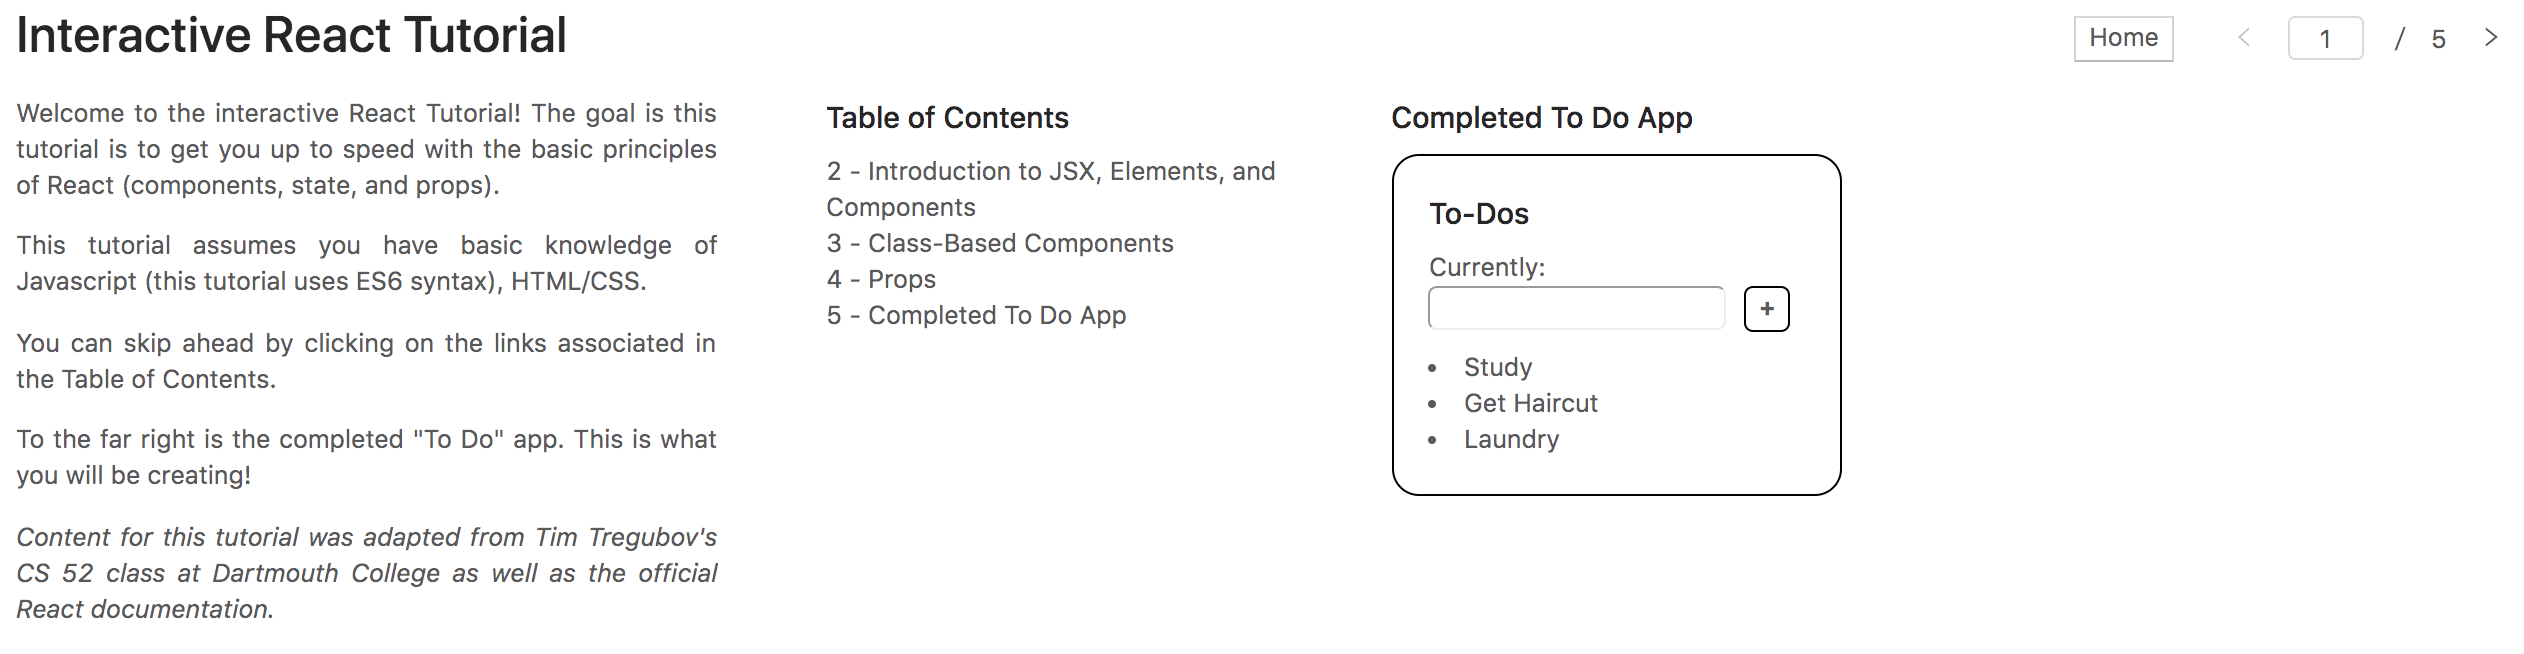
\includegraphics[scale=0.35]{homepage.png}
\end{center}

\figcaption{\textit{LearnReact}'s homepage. The homepage features (1) a table of contents in which each entry links to its corresponding module, and (2) an example of the completed application.}

\label{fig:Homepage}

\end{figure}

Currently, the modules range from basic concepts (such as introducing JSX and components) to harder concepts such as props and state. The beginning modules contain code that can be compiled with no edits, in order to show the user how components work. However, harder modules will have commented out sections where the user can fill in code. The commented out sections are designed to target key concepts associated with the module.

\begin{figure}[h]

\begin{center}
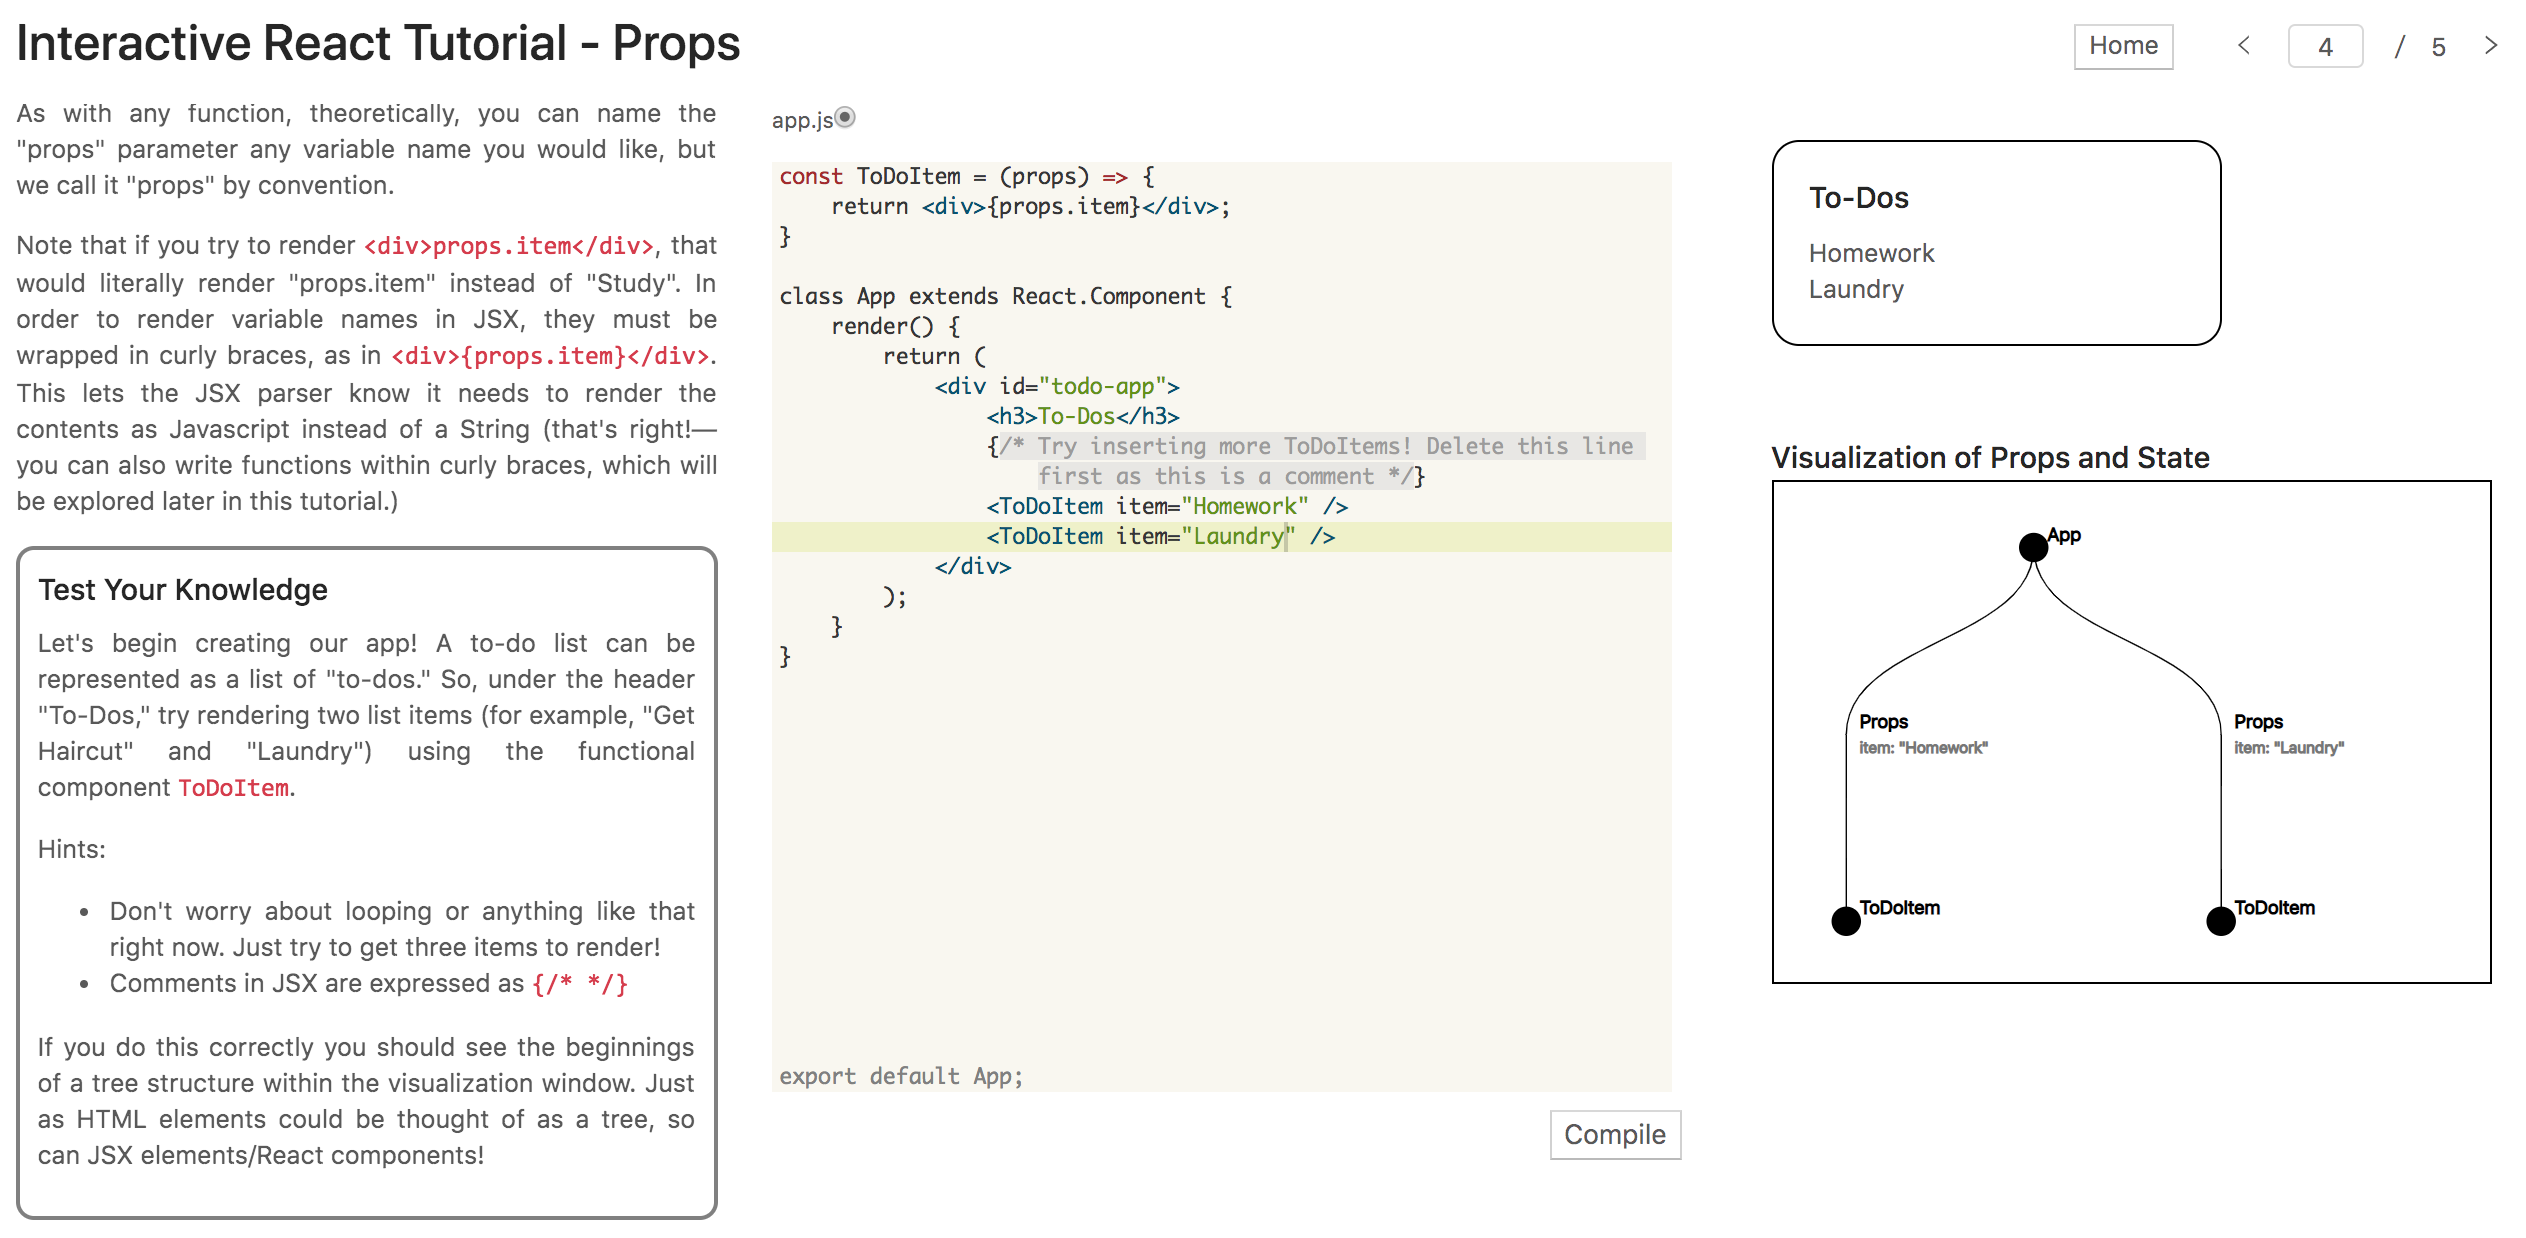
\includegraphics[scale=0.35]{module.png}
\end{center}

\figcaption{An example of a module. The left component contains text with describing the concepts as well as a exercise for the module. The center component is an IDE that allows the user to edit and compile React/Javascript code. The top-right component contains an in-progress example of the to-do application, and the bottom-right component is the visualization of props and state.}

\label{fig:Module}

\end{figure}

\section{Architecture}

Currently, the project is built entirely in React and basic Javascript.

\subsection*{Modules}

The modules in the web application are designed to be customizable. This makes the system generalizable and insulated from future changes in React. The text of each module are stored as an array of JSON objects that describe each module. The indices of the array correspond to the order in which modules appear. The important fields for each JSON object are ``title,'' ``instructions,'' and ''code.'' These fields are rendered on the screen when the corresponding module is called. That way, module text and lessons are separate from the infrastructure of the project.

\subsection*{Code Execution}

Once the user presses \texttt{Compile}, the code from the IDE is compiled in the browser and returns a React object to be that can be directly rendered (i.e., the actual to-do application). The compilation process is relatively straightforward: the code is linted (checked for obvious human errors), edited to extract props and state (this is for visualization and will be further discussed in the \textit{Visualization} subsection), and then converted to a React object. The created React object is then rendered by replacing the \texttt{\textless div\textgreater} element with the specified ID.

\subsection*{Visualization}

The bulk of the visualization is rendered using the \textit{D3.js} visualization library \cite{d3}. The library allows creating nodes and edges in order to depict the graph, but the associated text (i.e. nodes, which represent components; edges, which represent passed down props; and bullet points, which represents state) must be scraped.

Scraping the user's code happens in the processing stage. After the user's code is linted to ensure the code runs and produces a viable React element, a \textit{higher-order component} (HOC) is wrapped around the element in order to grab the props. To clarify, the higher-order component takes in the incoming props of the parent component, saves the props in the HOC state, and renders the wrapped component as a child. Importantly, the higher-order component does not modify any of the wrapped component's code and is only needed to grab the incoming props. The method for grabbing state is less elegant, however. To grab state, the user's code is first scanned to see if it is a stateful component. If it is, then the state variables are grabbed. However, this is prone to error and does not update as the local state changes.

To our knowledge, this described technique of scraping information from the app components to depict a visualization has not been done before in other tutorials. Depicting a React application's props and states in a graph visualization is not novel, however. Some Google Chrome extensions have attempted to scrape an application in order to build a tree \cite{reactsight} \cite{reactide}, but no prior projects have injected the visualization in a tutorial with an in-browser IDE. Thus, the ability to visualize how props and state interact is what sets our application apart from other tutorials.

\section{Future Work}

\subsection*{Planned Features}

Currently, the application is still in development. However, we shall implement the following features.

\subsubsection*{Persisting to a Database}

The web application does not save any user or user-associated data. For example, as users follow through the tutorial, they may find it helpful to keep track of their progress on a module or log into an account and see their previous code. The app is currently set up such that if users navigate away from a module and back to it, the module automatically resets to default. In addition, though the modules connect to build a to-do application, the users fill in blocks of code, rather than actually having a single project they work on. Therefore, we plan to implement a backend database to keep track of the user's progress.

The database shall be a MongoDB database hosted on Heroku, and backend scripting will be written in Javascript using the Mongoose framework. With the Mongoose framework, we plan to implement only one schema (i.e., table): users. Fields for the user table will be username and password (in encrypted form), and current code. Currently, we plan to implement three API points in the backend server: \textit{sign up} to sign up new users, \textit{sign in} to sign in existing users, and \textit{save code} to save the user's current code.

Of course, these changes may result in changing some parts of the frontend setup. Some changes may include adding in a sign up or sign in option in the navigation bar. Additionally, figuring out how to reconcile the current lesson plan structure with the users' code would also be a challenge, as the user's code could diverge significantly from the instructions and exercises the modules present.

\subsubsection*{Customizing Styles}

There is no way to customize the styles, or look, of the to-do application. Currently, the user must follow a set of styles that are already built into the webpage. So, when they are building new components, they need to use the styles provided by the web application. This limitation may confuse the user, especially if they are new to web development and do not have a solid understanding of CSS. Additionally, the user may not want to follow the style of the pre-defined to-do application and instead style the app to their own liking.

Thus, we plan to add another editor to exclusively handle styles. With this editor, users will be able to write their own CSS files to style their application. Thus, users can write their own pre-defined IDs and classes to style their application accordingly.

\subsection*{Limitations}

\subsubsection*{Fixed ``To-Do'' Application}

Components are currently not generalizable. That is, the app forces a to-do application to be built. So, if users want to build any other type of application using the tutorial, they would not be able to. At first glance, this may not be that large of an issue, as the web application is focused on being an introduction to learning React. A simple to-do application is also one of the easiest web applications to build, so the relationship between components, props, and state would be more digestible.

Under the current setup, however, users would not be able to code their own applications in a sandbox environment. This limitation also undermines the visualization feature, for React applications often have components nested inside components. While the visualization currently can depict a relationship between the parent and the child, the application cannot show relationships between grandparents and children, as there are only two layers of components in this application. This issue could be fixed in the future, but much of the application is written around the to-do application, and could introduce other unforeseen bugs.

\section{Conclusion}

We feel the web application offers two major advantages over online guides and similar interactive tutorials. The first is that the modules are designed to be separate from the infrastructure of the app, so new modules can be developed as the React library matures. If a generalizable components feature were to be implemented, then this flexibility could also be expanded to provide a general framework for creating lesson plans.The second advantage is providing the visualization of props and state, for this type of visualization has not been found in other online tutorials.

We are still developing the application at time of writing, so we were unable to gather formal or significantly quantifiable data. Anecdotally, students in CS 52 who we have tested the application on appreciated the current features and remarked that the application would have been helpful while learning the technology. Thus, we are optimistic that this application can help.

% \section{Related Work}

\section{Appendix}

\subsection*{Basic React Concepts}

Though the application is a tutorial on React, the application is actually built using the React framework. Thus, if you are unfamiliar with React, then you may find it difficult following the paper (especially sections on architecture and future work). Thus, I include an appendix to focus on main concepts.

\subsubsection*{Elements and Components}

Elements are the building blocks of React. An element describes what you want to see on the screen using JSX syntax. JSX syntax looks like HTML, but you can think of it as an add-on to Javascript that makes it easier to describe what you want rendered on the screen. An application built in React is composed of many components, which in return are composed of React elements. In React, components are actually just functions. They accept inputs, called props, and return React elements to be displayed.

\subsubsection*{Props}

In React, components are organized in a tree structure. An application is a parent component that is comprised of child components, which in turn may also be parent components to their own child components. The way parents communicate to children is via objects called \textit{props}. A props object may contain variables (variables that you want the child component to use) and/or functions (functions that are defined and bound to a parent component, but used by the parent's child component).

\subsubsection*{State}

Whereas props are variables that are shared between parent and components, state variables are variables that keep track of a component's local state. They are usually defined when a component is mounted and updated while the component is active. Typically state variables contain data that pertain to only the component and are not shared from parent to child.

\subsection*{Code}

The repository for the project can be accessed at \textit{https://github.com/byang18/react-tutorial}. The link to the web application is \textit{https://byang18.github.io/react-tutorial/}.

% props and state
% components

% generalizable components
% saving user project via a custom online database -- security requirements

%\bibliographystyle{abbrv}
%\bibliography{main}
\newpage
\bibliography{bib}
\bibliographystyle{ieeetr}

\end{document}
  